\documentclass[10pt]{article}
\usepackage[letterpaper]{geometry}
\geometry{verbose,tmargin=1in,bmargin=1in,lmargin=1in,rmargin=1in}
\usepackage{setspace}
\usepackage{ragged2e}
\usepackage{color}
\usepackage{titlesec}
\usepackage{graphicx}
\usepackage{float}
\usepackage{mathtools}
\usepackage{amsmath}
\usepackage[font=small,labelfont=bf,labelsep=period]{caption}
\usepackage[english]{babel}
\usepackage{indentfirst}
\usepackage{array}
\usepackage{makecell}
\usepackage[usenames,dvipsnames]{xcolor}
\usepackage{multirow}
\usepackage{tabularx}
\usepackage{arydshln}
\usepackage{caption}
\usepackage{subcaption}
\usepackage{xfrac}
\usepackage{etoolbox}
\usepackage{cite}
\usepackage{url}
\usepackage{dcolumn}
\usepackage{hyperref}
\usepackage{courier}
\usepackage{url}
\usepackage{esvect}
\usepackage{commath}
\usepackage{verbatim} % for block comments
\usepackage{enumitem}
\usepackage{hyperref} % for clickable table of contents
\usepackage{braket}
\usepackage{titlesec}
\usepackage{booktabs}
\usepackage{gensymb}
\usepackage{longtable}
\usepackage{listings}
\usepackage{cancel}
\usepackage{tcolorbox}
\usepackage[mathscr]{euscript}
\lstset{
    frame=single,
    breaklines=true,
    postbreak=\raisebox{0ex}[0ex][0ex]{\ensuremath{\color{red}\hookrightarrow\space}}
}

% for circled numbers
\usepackage{tikz}
\newcommand*\circled[1]{\tikz[baseline=(char.base)]{
            \node[shape=circle,draw,inner sep=2pt] (char) {#1};}}

\newcommand{\beq}{\begin{equation}}
\newcommand{\eeq}{\end{equation}}
\newcommand{\beqa}{\begin{equation}\begin{aligned}}
\newcommand{\eeqa}{\end{aligned}\end{equation}}

\titleclass{\subsubsubsection}{straight}[\subsection]

% define new command for triple sub sections
\newcounter{subsubsubsection}[subsubsection]
\renewcommand\thesubsubsubsection{\thesubsubsection.\arabic{subsubsubsection}}
\renewcommand\theparagraph{\thesubsubsubsection.\arabic{paragraph}} % optional; useful if paragraphs are to be numbered

\titleformat{\subsubsubsection}
  {\normalfont\normalsize\bfseries}{\thesubsubsubsection}{1em}{}
\titlespacing*{\subsubsubsection}
{0pt}{3.25ex plus 1ex minus .2ex}{1.5ex plus .2ex}

\makeatletter
\renewcommand\paragraph{\@startsection{paragraph}{5}{\z@}%
  {3.25ex \@plus1ex \@minus.2ex}%
  {-1em}%
  {\normalfont\normalsize\bfseries}}
\renewcommand\subparagraph{\@startsection{subparagraph}{6}{\parindent}%
  {3.25ex \@plus1ex \@minus .2ex}%
  {-1em}%
  {\normalfont\normalsize\bfseries}}
\def\toclevel@subsubsubsection{4}
\def\toclevel@paragraph{5}
\def\toclevel@paragraph{6}
\def\l@subsubsubsection{\@dottedtocline{4}{7em}{4em}}
\def\l@paragraph{\@dottedtocline{5}{10em}{5em}}
\def\l@subparagraph{\@dottedtocline{6}{14em}{6em}}
\makeatother

\newcommand{\volume}{\mathop{\ooalign{\hfil$V$\hfil\cr\kern0.08em--\hfil\cr}}\nolimits}

\setcounter{secnumdepth}{4}
\setcounter{tocdepth}{4}
\begin{document}

\title{MATH 228b: HW2}
\author{April Novak}

\maketitle

Note: The Professor's version of {\tt pmesh.m} is used for this assignment instead of my own from HW 1 because I got points off (I presume) due to my meshing. 

\section{} 

The solution of the following problem with linear Lagrange elements for \(u(0)=0\) and \(u'(1)=g\) is equivalent to a second order central difference approximation of the problem. 

\beq
\label{eq:1}
-u''(x)=f(x)
\eeq

The function space for the weight function \(v\) is in the space \(V_h\) such that \(v\) is \(C^0\) continuous over the entire domain (the zeroth derivative is the highest continuous derivative), where over each element \(K\), \(v\) is a linear function. \(v\) satisfies the homogeneous form of the Dirichlet boundary condition.

\beq
V_h=\{v\in C^0([0,1]): v\rvert_K\in P_1(K) \forall K\in T_h, v(0)=0\}
\eeq

The weighted residual form is obtained by multiplying Eq. \eqref{eq:1} by \(v\) and integrating over the domain. The first term on the left-hand side can be rewritten using the divergence rule:

\beqa
-\int_0^1 u''(x)v(x)dx=& \int_0^1 f(x)v(x)dx
\int_0^1 u'(x)v'(x)dx-\left\lbrack u'(x)v(x)\right\rbrack_0^1=& \int_0^1 f(x)v(x)dx
\eeqa

At this point, the weighted residual form has been reduced to the weak form. The weak form above contains no information about the boundary conditions. By applying the boundary conditions, the above reduces to:

\beq
\int_0^1 u'(x)v'(x)dx=\int_0^1 f(x)v(x)dx+gv(1)
\eeq

Using a linear Lagrange basis, defined on a mesh with element sizes \(h\), the elements are defined on \(e^1: [0, h]; e^2: [h, 2h]; e^3: [3h, 4h]; \cdots; e^n: [1-h, h]\), where \(n\) is the number of elements. The left and right coordinates of each element will be denoted as \(x_i\) and \(x_{i+1}\) for simplicity. Then, over an arbitrary element, the linear Lagrange shape functions \(\psi\) are:

\beqa
\psi_i(x)=& \frac{x_{i+1}-x}{x_{i+1}-x_i}=\frac{x_{i+1}-x}{h}\\
\psi_{i+1}(x) =& \frac{x-x_i}{x_{i+1}-x_i}=\frac{x-x_i}{h}\\
\eeqa

And their derivatives with respect to \(x\) are:

\beqa
\psi_i'(x)=&-\frac{1}{h}\\
\psi_{i+1}'(x) =&\frac{1}{h}\\
\eeqa

For equal-sized elements without edges on the Neumann boundary, the element stiffness matrix and element load vector are given as:

\beqa
A_{ij}^k=&\int_{x_i}^{x_{i+1}}\psi_i'(x)v_j'(x)dx\\
f_j^k=&\int_{x_i}^{x_{i+1}}f(x)v_j(x)dx\\
\eeqa

By inserting the shape functions given above, \(\textbf{A}^k\) becomes:

\beqa
\textbf{A}^k=& \begin{bmatrix}	\int_{x_i}^{x_{i+1}}\frac{-1}{h}\frac{-1}{h}dx & 
										\int_{x_i}^{x_{i+1}}\frac{-1}{h}\frac{1}{h}dx\\
										\int_{x_i}^{x_{i+1}}\frac{1}{h}\frac{-1}{h}dx &
										\int_{x_i}^{x_{i+1}}\frac{1}{h}\frac{1}{h}dx
					\end{bmatrix}\\
			   =& \begin{bmatrix}	1/h & 
										-1/h\\
										-1/h &
										1/h
					\end{bmatrix}
\eeqa

And the load vector becomes, with \(f=1\) chosen for simplicity:

\beqa
\textbf{f}^{\ k}=& \begin{bmatrix}	\int_{x_i}^{x_{i+1}}\frac{x_{i+1}-x}{h}dx \\
										\int_{x_i}^{x_{i+1}}\frac{x-x_i}{h}dx
					\end{bmatrix}\\
			   =& \begin{bmatrix}	\frac{(x_{i+1}-x_i)^2}{2h}\\
										\frac{(x_{i+1}-x_i)^2}{2h}
					\end{bmatrix}\\
				=& \begin{bmatrix}	h/2\\ 
										h/2
					\end{bmatrix}
\eeqa

Then, by the connectivity matrix relating how the nodes touch each other, the above matrices are ``tesselated'' along the diagonal of the global \textbf{A} and \textbf{f}. Suppose for the time being that \(u(1)=0\), i.e. both ends have homogeneous Dirichlet conditions. Then, the matrix system before application of the Dirichlet conditions is:

\beqa
\label{eq:3}
\begin{bmatrix}
1/h & -1/h & & & & &\\
-1/h & 2/h & -1/h & & & & \\
 & -1/h & 2/h & -1/h & & & \\
 & & -1/h & 2/h & -1/h & & \\
 & & & & & &\\
\end{bmatrix}
\begin{bmatrix}u_1\\u_2\\\vdots\\u_{n+1}\end{bmatrix} = 
\begin{bmatrix}
h/2\\ h\\h\\\vdots\\h\\h/2
\end{bmatrix}
\eeqa

Now, to apply the Neumann condition at \(x=1\), the load vector for the last element (the element spanning \(1-h\leq x\leq1\) must be modified:

\beqa
\textbf{f}^{\ e=n}=& \begin{bmatrix}	\int_{x_i}^{x_{i+1}}\frac{x_{i+1}-x}{h}dx \\
										\int_{x_i}^{x_{i+1}}\frac{x-x_i}{h}dx+g
					\end{bmatrix}\\
			   =& \begin{bmatrix}	\frac{(x_{i+1}-x_i)^2}{2h}\\
										\frac{(x_{i+1}-x_i)^2}{2h}+g
					\end{bmatrix}\\
				=& \begin{bmatrix}	h/2\\ 
										h/2+g
					\end{bmatrix}
\eeqa

Then, the last equation in Eq. \eqref{eq:3} must be modified. To strongly apply the homogeneous Dirichlet condition at \(x=0\), the first row and column of \textbf{A} is eliminated, and post-processing will assign the value \(u_1=0\). The full matrix system, with boundary conditions \(u(0)=0, u'(1)=g\), is, for a four-element system (purely for illustration):

\beqa
\label{eq:3}
\begin{bmatrix}
 2/h & -1/h & 0 & 0 \\
 -1/h & 2/h & -1/h & 0 \\
 0 & -1/h & 2/h & -1/h\\
 0 & 0 & -1/h & 1/h\\
\end{bmatrix}
\begin{bmatrix}u_2\\u_3\\u_4\\u_5\end{bmatrix} = 
\begin{bmatrix}
h\\h\\h\\h/2+g
\end{bmatrix}
\eeqa

Divide both sides by \(h\) for future insight into our choice of \(f(x)=1\):

\beqa
\label{eq:3}\frac{1}{h^2}
\begin{bmatrix}
 2 & -1 & 0 & 0 \\
 -1 & 2 & -1 & 0 \\
 0 & -1 & 2 & -1\\
 0 & 0 & -1 & 1\\
\end{bmatrix}
\begin{bmatrix}u_2\\u_3\\u_4\\u_5\end{bmatrix} = 
\begin{bmatrix}
1\\1\\1\\(h/2+g)/h
\end{bmatrix}
\eeqa

The central difference approximation to a second derivative is:

\beq
u''(x)\approx \frac{u_{i+1}-2u_i+u_{i-1}}{h^2}
\eeq

Looking at the equation for node 3, for instance, we can express this equation for \(i=3\) in terms of the values on either side (\(u_2=u_{i-1}\) and \(u_4=u_{i+1}\)):

\beq
\label{eq:4}
-\frac{1}{h^2}\left(u_{i-1}-2u_i+u_{i+1}\right)=1
\eeq

Eq. \eqref{eq:4} is identical to central difference approximation of the original equation in Eq. \eqref{eq:1} - the second derivative is approximated as a central difference, while the right-hand-side reflects the (arbitrary) choice of setting \(f(x)=1\). The above equation holds for all nodes on the interior. The enforcement of the Neumann condition can also be seen analogous to a finite difference approximation. The equation for the node on the Neumann boundary (node 5, where \(i=5\)), is:

\beq
\frac{1}{h}(-u_{i-1}+u_i)=\frac{h}{2}+g
\eeq

It is clear to see that the above represents a forward Euler method, since the slope at node \(i\) depends only on the solution value at \(i-1\). The \(h/2\) appears from the tessellation of the element load vector in \textbf{f}, and hence if that part is neglected for the time begin, then the above is exactly equivalent to stating that:

\beq
u'(1)\approx\frac{u_5-u_4}{h}=g+\frac{h}{2}f(x_{i-1})
\eeq

where the additional term on the right-hand side has been added as a correction term that results in a second-order approximation to the first derivative. So, this shows that, for linear Lagrange elements in 1-D, the finite element method is equivalent to a central difference method on the interior nodes with a second order finite difference method enforcing Neumann conditions on the boundaries through the use of a correction factor. So, for this simple case, the finite element method is equivalent to a second order finite difference approximation of the governing equation.

\section{}

This question will solve the following boundary value problem on \(x\in[0,1]\):

\beq
u''''(x)=f(x)=480x-120
\eeq

with boundary conditions \(u(0)=u'(0)=u(1)=u'(1)=0\). 

\subsection{}

The Galerkin formulation seeks a solution \(u_h\) in the function space \(V_h\), which is the same function space as the weight function \(v\):

\beq
V_h=\{v\in C^1([0,1]):v\rvert_K\in P_3(K) \forall K\in T_h, v(0)=v(1)=0=v'(0)=v'(1)\}
\eeq

The only requirement on the function space \(V_h\) is that it satisfy the homogeneous form of the essential boundary conditions. For a fourth-order governing equation, the essential boundary conditions are represented by the values of \(u\) and \(u'\) on the boundaries, while the natural boundary conditions in this case are the values of \(u'''\) and \(u''\) on the boundaries. In order for \(v\) to be able to satisfy the essential boundary conditions, \(v\) must be of sufficiently high order to specify \(v\) and \(v'\) on the boundaries (which for a 1-D element requires four degrees of freedom per element, neglecting continuity and boundary conditions requirements for the time being). Multiplying the governing equation by a weight function \(v(x)\) and integrating over the domain gives the weighted residual formulation of the governing equation:

\beq
\int_{0}^{1}u''''(x)v(x)dx=\int_{0}^{1}f(x)v(x)dx
\eeq

Integrating by parts two times:

\beqa
-\int_{0}^{1}u'''(x)v'(x)dx+\left\lbrack u'''(x)v(x)\right\rbrack_0^1=& \int_{0}^{1}f(x)v(x)dx\\
\int_{0}^{1}u''(x)v''(x)dx+\left\lbrack u'''(x)v(x)\right\rbrack_0^1-\left\lbrack u''(x)v'(x)\right\rbrack_0^1=& \int_{0}^{1}f(x)v(x)dx
\eeqa

Then, applying the boundary conditions:

\beq
\int_{0}^{1}u''(x)v''(x)dx=\int_{0}^{1}f(x)v(x)dx \quad\forall v\in V_h
\eeq

Now that differentiation has been modified to act equally (to the extent possible based on the governing equation) on \(u\) and \(v\), the above represents the weak form. The above equation holds for both the true solution \(u\) and the finite element solution \(u_h\), and hence the above could also be written as follows, which matches that shown in this homework assignment:

\beq
\int_{0}^{1}u_h''(x)v''(x)dx=\int_{0}^{1}f(x)v(x)dx \quad\forall v\in V_h
\eeq

\subsection{}

Over a particular element, the solution is specified as a summation of coefficients \(a\) multiplied by basis functions \(\varphi\), where \(N\) is the number of shape functions per element (which for linear Lagrange elements is equivalent to the number of nodes per element):

\beq
\label{eq:11}
u_h^e(x)=\sum_{i=1}^{N}a_i\varphi_i(x)
\eeq

The above expression uses an \(e\) in the superscript of \(u_h\) to refer to the fact that \(u_h^e\) is the solution only over a particular element \(e\) - we must find the solution over every element. Because the space is defined to contain cubic polynomials over each element, since we require four degrees of freedom per element (not yet assuming continuity between elements), the shape functions for this problem must be functions that can specify both types of essential boundary conditions - the value and the first derivative on the two boundary nodes for each element. This requires four shape functions per element. Hermite shape functions allow specification of both the value and derivative at edge nodes. There are four shape functions per element. These shape functions are defined over an element defined on \([a, b]\) as:

\beqa
\label{eq:5}
H_1(a)=1, H_1(b)=0, \frac{dH_1(a)}{dx}=0, \frac{dH_1(b)}{dx}=0\\
H_2(a)=0, H_2(b)=1, \frac{dH_2(a)}{dx}=0, \frac{dH_2(b)}{dx}=0\\
H_3(a)=0, H_3(b)=0, \frac{dH_3(a)}{dx}=1, \frac{dH_3(b)}{dx}=0\\
H_4(a)=0, H_4(b)=0, \frac{dH_4(a)}{dx}=0, \frac{dH_4(b)}{dx}=1\\
\eeqa

where \(H\) is used to represent the fact that these shape functions \(\psi\) are Hermite shape functions. For each of these shape functions, because they are cubic, they are uniquely represented by four coefficients \(c, d, e, f\) for a polynomial of the form:

\beqa
H_1(x)=&c_1x^3+d_1x^2+e_1x+f_1\\
H_2(x)=&c_2x^3+d_2x^2+e_2x+f_2\\
H_3(x)=&c_3x^3+d_3x^2+e_3x+f_3\\
H_4(x)=&c_4x^3+d_4x^2+e_4x+f_4\\
\eeqa

\beqa
\frac{dH_1(x)}{dx}=&3c_1x^2+2d_1x+e_1\\
\frac{dH_2(x)}{dx}=&3c_2x^2+2d_2x+e_2\\
\frac{dH_3(x)}{dx}=&3c_3x^2+2d_3x+e_3\\
\frac{dH_4(x)}{dx}=&3c_4x^2+2d_4x+e_4\\
\eeqa

So, for each element in the triangulation, these 16 coefficients must be determined by solving the following linear system for \textit{each} of the functions \(H_i\):

\beq
\begin{bmatrix}
a^3 & a^2 & a & 1\\
b^3 & b^2 & b & 1\\
3a^2 & 2a & 1 & 0\\
3b^2 & 2b & 1 & 0
\end{bmatrix}
\begin{bmatrix}
c_1 \\d_1 \\e_1 \\f_1
\end{bmatrix}
=
\begin{bmatrix}
1 \\ 0 \\ 0 \\ 0
\end{bmatrix}
\quad\quad \textrm{for } H_1
\eeq

\beq
\begin{bmatrix}
a^3 & a^2 & a & 1\\
b^3 & b^2 & b & 1\\
3a^2 & 2a & 1 & 0\\
3b^2 & 2b & 1 & 0
\end{bmatrix}
\begin{bmatrix}
c_2 \\d_2 \\e_2 \\f_2
\end{bmatrix}
=
\begin{bmatrix}
0 \\ 1 \\ 0 \\ 0
\end{bmatrix}
\quad\quad \textrm{for } H_2
\eeq

\beq
\begin{bmatrix}
a^3 & a^2 & a & 1\\
b^3 & b^2 & b & 1\\
3a^2 & 2a & 1 & 0\\
3b^2 & 2b & 1 & 0
\end{bmatrix}
\begin{bmatrix}
c_3 \\d_3 \\e_3 \\f_3
\end{bmatrix}
=
\begin{bmatrix}
0 \\ 0 \\ 1 \\ 0
\end{bmatrix}
\quad\quad \textrm{for } H_3
\eeq

\beq
\begin{bmatrix}
a^3 & a^2 & a & 1\\
b^3 & b^2 & b & 1\\
3a^2 & 2a & 1 & 0\\
3b^2 & 2b & 1 & 0
\end{bmatrix}
\begin{bmatrix}
c_4 \\d_4 \\e_4 \\f_4
\end{bmatrix}
=
\begin{bmatrix}
0 \\ 0 \\ 0 \\ 4
\end{bmatrix}
\quad\quad \textrm{for } H_4
\eeq

Then, this process is repeated for all the elements in the triangulation, where \(a\) and \(b\) will change corresponding to the endpoints of the domain. This system of equations is solved in Python, where the code is provided in the Appendix. This solution, for the two-element triangulation given, for superscripts that indicate the element number, is:

\beqa
H_1^1(x)=&16x^3-12x^2+1\\
H_2^1(x)=&-16x^3+12x^2\\
H_3^1(x)=&4x^3-4x^2+x\\
H_4^1(x)=&4x^3-2x^2\\
\eeqa

\beqa
H_1^2(x)=&16x^3-36x^2+24x-4\\
H_2^2(x)=&-16x^3+36x^2-24x+5\\
H_3^2(x)=&4x^3-10x^2+8x-2\\
H_4^2(x)=&4x^3-8x^2+5x-1\\
\eeqa

The second derivatives of these functions are needed for the finite element formulation, so they are computed as:

\beqa
\frac{d^2H_1^1(x)}{dx^2}=& 96x-24\\
\frac{d^2H_2^1(x)}{dx^2}=& -96x+24\\
\frac{d^2H_3^1(x)}{dx^2}=& 24x-8\\
\frac{d^2H_4^1(x)}{dx^2}=& 24x-4\\
\eeqa

\beqa
\frac{d^2H_1^2(x)}{dx^2}=& 96x-72\\
\frac{d^2H_2^2(x)}{dx^2}=& -96x+72\\
\frac{d^2H_3^2(x)}{dx^2}=& 24-20\\
\frac{d^2H_4^2(x)}{dx^2}=& 24-16\\
\eeqa

Fig. \ref{fig:1} shows the shape functions over the two-element domain. The basis over the domain is therefore these eight Hermite functions. These functions correspond to eight degrees of freedom, which are reduced to two when considering that the values and first derivatives at the single shared node must be continuous. Then, the four boundary conditions specify four of the degrees of freedom, leaving two degrees of freedom that are to be solved for using the finite element method. Because there are two degrees of freedom, the solution can be uniquely expressed as the sum of only two of these eight Hermite functions (this is specific to this particular problem). 

\begin{figure}[H]
\centering
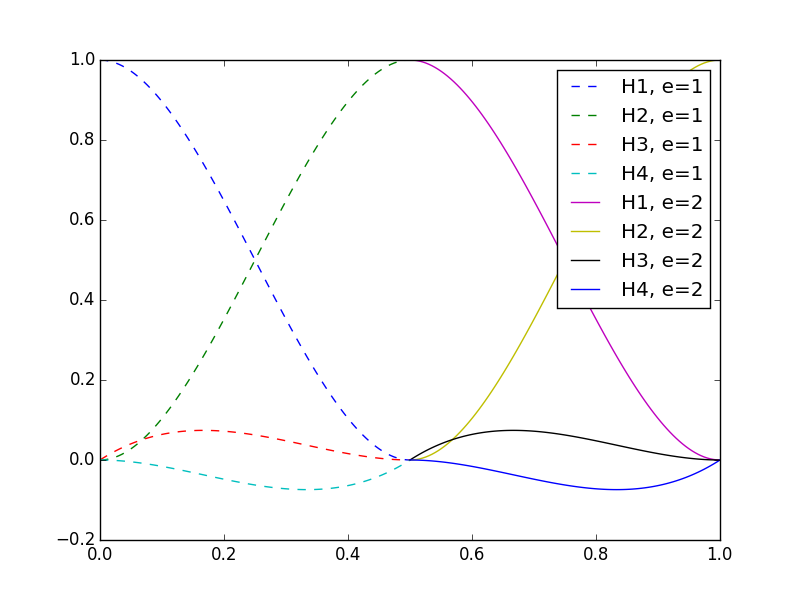
\includegraphics[width=0.75\textwidth]{q2_Hermite_functions.png}
\caption{Hermite shape functions over the two-element domain.}
\label{fig:1}
\end{figure}

\subsection{}

The elemental stiffness matrix is given by:

\beq
A_{ij}^k=\int_0^1\frac{d^2H_i^k(x)}{dx^2}\frac{d^2H_j^k(x)}{dx^2}dx
\eeq

The elemental load vector is given by:

\beq
f_j=\int_{0}^{1}f(x)H_j^k(x)dx
\eeq

For element 1:

\beq
\textbf{A}^1=\begin{bmatrix}
\int_{0}^{0.5}\frac{d^2H_1^1(x)}{dx^2}\frac{d^2H_1^1(x)}{dx^2}dx & \int_{0}^{0.5}\frac{d^2H_1^1(x)}{dx^2}\frac{d^2H_2^1(x)}{dx^2}dx & \int_{0}^{0.5}\frac{d^2H_1^1(x)}{dx^2}\frac{d^2H_3^1(x)}{dx^2}dx & \int_{0}^{0.5}\frac{d^2H_1^1(x)}{dx^2}\frac{d^2H_4^1(x)}{dx^2}dx\\
\int_{0}^{0.5}\frac{d^2H_2^1(x)}{dx^2}\frac{d^2H_1^1(x)}{dx^2}dx & \int_{0}^{0.5}\frac{d^2H_2^1(x)}{dx^2}\frac{d^2H_2^1(x)}{dx^2}dx & \int_{0}^{0.5}\frac{d^2H_2^1(x)}{dx^2}\frac{d^2H_3^1(x)}{dx^2}dx & \int_{0}^{0.5}\frac{d^2H_2^1(x)}{dx^2}\frac{d^2H_4^1(x)}{dx^2}dx\\
\int_{0}^{0.5}\frac{d^2H_3^1(x)}{dx^2}\frac{d^2H_1^1(x)}{dx^2}dx & \int_{0}^{0.5}\frac{d^2H_3^1(x)}{dx^2}\frac{d^2H_2^1(x)}{dx^2}dx & \int_{0}^{0.5}\frac{d^2H_3^1(x)}{dx^2}\frac{d^2H_3^1(x)}{dx^2}dx & \int_{0}^{0.5}\frac{d^2H_3^1(x)}{dx^2}\frac{d^2H_4^1(x)}{dx^2}dx\\
\int_{0}^{0.5}\frac{d^2H_4^1(x)}{dx^2}\frac{d^2H_1^1(x)}{dx^2}dx & \int_{0}^{0.5}\frac{d^2H_4^1(x)}{dx^2}\frac{d^2H_2^1(x)}{dx^2}dx & \int_{0}^{0.5}\frac{d^2H_4^1(x)}{dx^2}\frac{d^2H_3^1(x)}{dx^2}dx & \int_{0}^{0.5}\frac{d^2H_4^1(x)}{dx^2}\frac{d^2H_4^1(x)}{dx^2}dx\\
\end{bmatrix}
\eeq

The local stiffness matrix is computed in the same method for element 2, except that the integration bounds change from \([0, 0.5]\) to \([0.5, 1.0]\). It should be noted that the elemental basis functions are only nonzero over the particular element, so \(\textbf{A} ^k\) is the same for both elements 1 and 2. Performing the computation shown above, the elemental stiffness matrices are (where the numbering given previously for the Hermite shape functions is changed so that 1 and 2 correspond to functions that obtain values and derivatives of unity at the left side, whereas 3 and 4 are reserved for the right side):

\beq
\textbf{A}^1=\textbf{A}^2=\begin{bmatrix}
96 & 24 & -96 & 24\\
24 & 8 & -24 & 4\\
-96 & -24 & 96 & -24\\
24 & 4 & -24 & 8\\
\end{bmatrix}
\eeq

And the elemental load vectors are:

\beqa
\textbf{f}^{\ 1}=\begin{bmatrix}-12 -0.5 12 -0.5\end{bmatrix}^T\\
\textbf{f}^{\ 2}=\begin{bmatrix}48 &4.5 & 72 & -5.5\end{bmatrix}^T
\eeqa

And the global system to be solved is:

\beq
\begin{bmatrix}
96 & 24 & -96 & 24 & 0 & 0\\
24 & 8 & -24 & 4 & 0 & 0\\
-96 & -24 & 96+96 & -24+24 & -96 & 24\\
24 & 4 & -24+24 & 8+8 &-24 & 4\\
0 & 0 & -96 & -24 & 96 & -24\\
0 & 0 & 24 & 4 & -24 & 8
\end{bmatrix}
\begin{bmatrix}
u_1\\u_2\\u_3\\u_4\\ u_5\\ u_6
\end{bmatrix}
=
\begin{bmatrix}
-12 \\-0.5 \\12+48 \\-0.5+4.5\\ 72\\-5.5
\end{bmatrix}
\eeq

This is not the final system that is solved, however, since the essential boundary conditions must be taken into account in this formulation. The matrix system to be solved can be broken up into:

\beq
\begin{bmatrix}
A_{uu} & A_{uk}\\
A_{ku} & A_{kk}
\end{bmatrix}
\begin{bmatrix}
u_u \\ u_k
\end{bmatrix} =
\begin{bmatrix}
f_u \\ f_k
\end{bmatrix}
\eeq

where the \(u\) and \(k\) subscripts indicate unknown (non-essential boundary condition locations) and known (essential boundary condition locations) values. So, instead of solving \(\textbf{A}\textbf{u}=\textbf{f}\) using the full matrices above, the following system must be solved:

\beq
A_{uu}u_u=f_u-A_{uk}x_k
\eeq

where \(x_k=\textbf{0}\) because all of the essential boundary conditions are homogeneous. From the boundary conditions, \(u_1=u_2=u_5=u_6=0\). So, the actual matrix system to be solved is:

\beq
\begin{bmatrix} 192 & 0\\
0 & 16
\end{bmatrix}
\begin{bmatrix} u_3\\u_4
\end{bmatrix}
=\begin{bmatrix} 60\\ 4\end{bmatrix}
\eeq

Solving this system gives \(u_3=5/16, u_4=1/4\), which then specifies the solution over the two elements according to Eq. \eqref{eq:11}:

\beqa
u_h^1(x)=& u_3(-16x^3-12x^2+1)+u_4*4x^3-2x^2\\
u_h^2(x)=& u_3(16x^3-36x^2+24x-4)+u_4(4x^3-10x^2+8x-2)\\
\eeqa

The analytical solution to the governing equation is given by:

\beqa
u(x)=&C_4x^3+C_3x^2+C_2x+C_1+4x^5-5x^4\\
u'(x)=&3C_4x^2+2C_3x+C_2+20x^4-20x^3\\
\eeqa

Applying the boundary conditions to determine the unknown coefficients gives \(C_1=0, C_2=0, C_3=3, C_4=-2\), so the analytical solution is:

\beq
u(x)=-2x^3+3x^2+4x^5-5x^4
\eeq

Fig. \ref{fig:2} shows a comparison between the analytical solution above and the finite element solution. As can be seen, the finite element solution is a fairly good approximation to the true solution, and had there been more elements, would have much better approximated the true solution. The code developed for this section is included in the Appendix.

\begin{figure}[H]
\centering
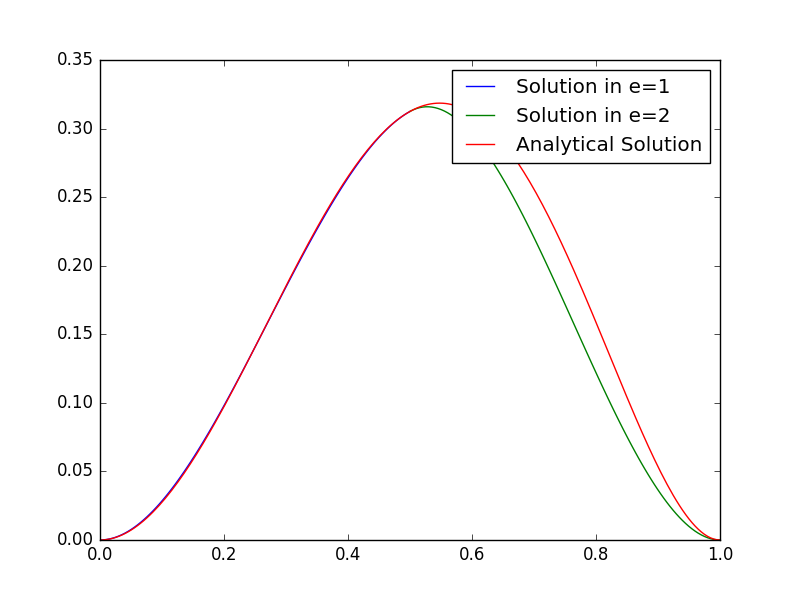
\includegraphics[width=0.75\textwidth]{q3_soln.png}
\caption{Comparison between the analytical and finite element solutions for the given problem statement.}
\label{fig:2}
\end{figure}

\section{}

This question solves the Poisson equation on an unstructured, triangular grid, subject to homogeneous Dirichlet and Neumann boundary conditions:

\beqa
-\nabla^2u(x,y)=1\\
u\rvert_{\Gamma_d}=0,\quad \hat{n}\cdot\nabla u\rvert_{\Gamma_t}=0\\
\eeqa

where \(\Gamma_d\) indicates the Dirichlet portion of the boundary and \(\Gamma_t\) the Neumann portion of the boundary, and \(\Gamma_d\cup\Gamma_t=\Gamma\). The weighted residual form is obtained by multiplying the above by a weight function \(v\):

\beq
-\int_\Omega \nabla^2u(x,y)v(x,y)d\Omega=\int_\Omega v(x,y)d\Omega
\eeq

The weak form is obtained by integrating by parts:

\beq
\int_\Omega \nabla u(x,y)\cdot\nabla v(x,y)d\Omega-\int_\Gamma\hat{n}\cdot\nabla u(x,y)v(x,y)d\Gamma=\int_\Omega v(x,y)d\Omega
\eeq

Homogeneous Neumann conditions allow the boundary term above to simply be dropped, since \(\hat{n}\cdot\nabla u(x,y)=0\) on \(\Gamma_t\) and the weight function \(v(x,y)\) satisfies the homogeneous form of the essential boundary conditions on the essential boundaries such that \(v(x,y)=0\) for all remaining parts of the boundary (since \(\Gamma_d\cap\Gamma_t=\emptyset\)). After removing this term, the following represents the weak form for the problem, where processing of the global stiffness matrix and global load vector are required to ensure that the solution obtains the specified values on the Dirichlet boundaries.

\beq
\int_\Omega \nabla u(x,y)\cdot\nabla v(x,y)d\Omega=\int_\Omega v(x,y)d\Omega
\eeq

\(u\) is approximated as \(u_h\) by expanding it in a series of basis functions \(\psi\):

\beq
u_h=\sum_{i=1}^{N}a_j\psi_j(x,y)
\eeq

where \(N\) is the total number of basis functions, which for Lagrange elements is equivalent to the number of nodes in the domain. Instead of defining basis functions that exist over the entire domain, to improve the sparsity of the matrices involved, expand \(u_h\) in \(n_{en}\) basis functions over each finite element, where \(n_{en}\) are the number of nodes per element. 

\beq
u_h^k=\sum_{i=1}^{n_{en}}a_j\psi_j(x,y)=\textbf{N}\textbf{u}
\eeq

The right-hand side can be represented as two vectors, one containing the shape functions, and the other containing the expansion coefficients. 

\beq
\textbf{N}=\begin{bmatrix} \psi_1(x,y) & \psi_2(x,y) & \cdots & \psi_{n_{en}}\end{bmatrix}
\eeq

\beq
\textbf{u}=\begin{bmatrix} a_1 & a_2 & \cdots & a_{n_{en}}\end{bmatrix}^T
\eeq

Likewise, the weight function \(v\) can also be expanded in the same manner, but with different expansion coefficients \textbf{b}. The gradient of \(u_h\) is defined as:

\beq
\nabla u_h=\frac{\partial u_h}{\partial x}\hat{x}+\frac{\partial u_h}{\partial y}\hat{y}=\textbf{B}\textbf{u}
\eeq

where \textbf{B} is a deformation matrix that acts on the solution \textbf{u} to produce the effect of the gradient. 

\beq
\textbf{B}=\begin{bmatrix}
\frac{\partial\psi_1}{dx} & \frac{\partial\psi_2}{dx} & \cdots & \frac{\partial\psi_{n_en}}{dx}\\
\frac{\partial\psi_1}{dy} & \frac{\partial\psi_2}{dy} & \cdots & \frac{\partial\psi_{n_en}}{dy}\\
\end{bmatrix}
\eeq

Then, noting that the dot product of two vectors can be written as \(\textbf{a}\cdot\textbf{b}=\textbf{a}^T\textbf{b}\), the weak form becomes:

\beqa
\int_\Omega (\textbf{B}\textbf{u})^T(\textbf{B}\textbf{v})d\Omega=&\int_\Omega \textbf{N}\textbf{v}d\Omega\\
\int_\Omega \textbf{B}^T\textbf{u}^T(\textbf{B}\textbf{v})d\Omega=&\int_\Omega \textbf{N}\textbf{v}d\Omega\\
\int_\Omega \textbf{B}^T\textbf{u}\textbf{B}d\Omega=&\int_\Omega \textbf{N}d\Omega\\
\eeqa

where \textbf{v} has essentially been cancelled from every term (the above could be rearranged such that \textbf{v} acts on an integrand, where the entire term equals zero such that the integrand must therefore equal zero). The above is essentially equivalent to the 1-D form, where \textbf{B} would reduce to \(d\psi_i/dx\) and \textbf{N} to \(\psi_i\). The elemental stiffness matrix and elemental load vector are:

\beq
\label{eq:20}
\textbf{A}^k=\int_{\Omega_k} \textbf{B}^T\textbf{B}d\Omega
\eeq

\beq
\label{eq:21}
\textbf{F}^k=\int_{\Omega_k} \textbf{N}d\Omega
\eeq

In order to apply over an individual element, the shape functions that appear in \textbf{B} and \textbf{N} must be the shape functions over that particular element. This can be achieved either by determining the shape functions over each element in the physical domain (in which case the shape functions are different for every element) or by using isoparametric elements that are mapped from a master domain, where the integrals above are always the same, and then modify the above terms with a Jacobian of the transformation. If these shape functions are determined individually for each element, they would be determined by solving the following system for the three different right-hand sides shown below to give the coefficients \(a, b, c\) for each of the three shape functions (assuming triangular elements for this problem):

\beq
\begin{bmatrix} x_1 & y_1 & 1\\x_2 & y_2 & 1\\x_3 & y_3 & 1\end{bmatrix}
\begin{bmatrix}a\\ b\\ c\end{bmatrix}=\begin{bmatrix}1\\ 0\\ 0\end{bmatrix};\ \begin{bmatrix}0\\ 1\\ 0\end{bmatrix};\ \begin{bmatrix}0\\ 0\\ 1\end{bmatrix}
\eeq

where \(x_i, y_i\) is the \(i\) coordinate of the triangle, for \(i=1, 2, 3\). Performing this for every triangle individually is tedious, and likewise determining the appropriate bounds of integration for each triangle is problematic and difficult when only the coordinate points are known. To overcome this, a mapping is performed from a master triangle with corners at \((0,0), (1,0), (0,1)\) in a coordinate system defined in terms of variables \(\xi\) and \(\eta\). The shape functions in this master domain will therefore be the same over each element in the physical domain, and the only thing that differs for each element is the Jacobian of the transformation. With \((x_1=0, y_1=0, (x_2=1, y_2=0), (x_3=0,y_3=1)\), the shape functions in the master domain are:

\beqa
\psi_1(\xi,\eta)=&1-\xi-\eta\\
\psi_2(\xi,\eta)=&\xi\\
\psi_3(\xi,\eta)=&\eta\\
\eeqa

The mapping from the master to physical domain is performed using an isoparametric mapping that relates the physical coordinates \((X_i,Y_i)\) to the master domain coordinates \((\xi,\eta)\)

\beqa
x(\xi,\eta)=&\sum_{i=1}^{n_{en}}X_i\psi_i(\xi,\eta)\\
y(\xi,\eta)=&\sum_{i=1}^{n_{en}}Y_i\psi_i(\xi,\eta)\\
\eeqa

To transform the integrals appearing in Eq. \eqref{eq:20} and \eqref{eq:21} to integrals over the master domain requires the use of the derivatives with respect to \(\xi\) and \(\eta\), rather than with respect to \(x\) and \(y\). The domain of integration changes according to:

\beqa
d\vv{x}=&\textbf{D}d\vv{\xi}\\
\begin{bmatrix}dx\\dy\end{bmatrix}=&
\begin{bmatrix}dx/d\xi & dx/d\eta\\ dy/d\xi & dy/d\eta\end{bmatrix}
\begin{bmatrix}d\xi\\d\eta\end{bmatrix}
\eeqa

where \textbf{D} is the transformation matrix that describes how the coordinate transformation is performed. The derivatives appearing in \textbf{D} are computed based on the definitions of the isoparametric mapping:

\beqa
\frac{dx(\xi,\eta)}{d\xi}=&\sum_{i=1}^{n_{en}}X_i\frac{d\psi_i(\xi,\eta)}{d\xi}\\
\frac{dx(\xi,\eta)}{d\eta}=&\sum_{i=1}^{n_{en}}X_i\frac{d\psi_i(\xi,\eta)}{d\eta}\\
\frac{dy(\xi,\eta)}{d\xi}=&\sum_{i=1}^{n_{en}}Y_i\frac{d\psi_i(\xi,\eta)}{d\xi}\\
\frac{dy(\xi,\eta)}{d\eta}=&\sum_{i=1}^{n_{en}}Y_i\frac{d\psi_i(\xi,\eta)}{d\eta}\\
\eeqa

With these definitions, the local stiffness matrix and local load vector transform to integrals over \(\xi, \eta\):

\beq
\label{eq:20}
\textbf{A}^k=\int_{0}^{1} \int_{0}^{1-\xi}(\textbf{D}^{-1}\textbf{C})^T(\textbf{D}^{-1}\textbf{C})|\textbf{D}| d\eta d\xi
\eeq

\beq
\label{eq:21}
\textbf{F}^k=\int_{0}^{1} \int_{0}^{1-\xi}\textbf{N}|\textbf{D}| d\eta d\xi
\eeq

where \textbf{C} is the same as \textbf{B}, except that derivatives are taken with respect to \(\xi\) and \(\eta\) instead of \(x\) and \(y\):

\beq
\textbf{C}=\begin{bmatrix}
\frac{\partial\psi_1}{d\xi} & \frac{\partial\psi_2}{d\xi} & \cdots & \frac{\partial\psi_{n_en}}{d\xi}\\
\frac{\partial\psi_1}{d\eta} & \frac{\partial\psi_2}{d\eta} & \cdots & \frac{\partial\psi_{n_en}}{d\eta}\\
\end{bmatrix}
\eeq

Note that the integrals in Eq. \eqref{eq:20} and \eqref{eq:21} are no longer over the domain of an element in the physical domain - they are over a triangle in the master domain. To allow easy calculation of these integrals without the need to use symbolic integration or the need to hard-code in the integrals given that all of the shape functions are linear in \(x\) and \(y\) (to permit faster extension to higher-order elements), quadrature rules are used to numerically evaluate the integrals above. A second motivation to using the transformation to the master domain is the ability to use the same quadrature rule over every element. Quadrature rules for the standard triangle defined with corners at \((0,0), (1,0), (0,1)\) are attempting to determine the weights \(w_i\) and quadrature points \(\xi_i,\eta_i\) so that the following summation is as accurate as possible for a polynomial of some given order:

\beq
\int_{0}^{1} \int_{0}^{1-\xi}f(\xi,\eta)d\eta d\xi\approx\sum_{i=1}^{n_{qp}}w_if(\xi_i,\eta_i)
\eeq

For \(n_{qp}=1\), the following one-point rule exactly integrates linear integrands:

\beqa
w=&[1/2]\\
(\xi_i,\eta_i)=&[1/3, 1/3]
\eeqa

For \(n_{qp}=3\), the following one-point rule exactly integrates quadratic integrands:

\beqa
w=&[1/6; 1/6; 1/6]\\
(\xi_i,\eta_i)=&[1/6, 1/6; 2/3, 1/6; 1/6, 2/3]
\eeqa

Because the highest order expected in the integrands for this problem occurs in \textbf{F}, which has an integrand that is at most order 1, the one-point quadrature rule is used. The elemental stiffness matrix and elemental load vector are computed for each individual element. They are then assembled in the global matrix according to the connectivity matrix, which is conveniently provided as the triangulation returned by the {\tt delaunay} function. For example, with the following triangulation for a domain where each element has four nodes, the connectivity matrix, also called the location matrix (LM), would be:

\begin{equation}
\textbf{LM}=\begin{bmatrix}
1 & 2 & 5 & 4\\
2 & 3 & 6 & 5\\
4 & 5 & 8 & 7\\
5 & 6 & 9 & 8\\
\end{bmatrix}
\end{equation}

where the local nodes are numbered in a counterclockwise manner beginning from the bottom left node. Then, for example, the second row in the global stiffness matrix would be assembled as:

\begin{equation}
\textbf{K}(2,:)=\begin{bmatrix}
k_{2,1}^{e=1}, & k_{2,2}^{e=1}+k_{1,1}^{e=2}, & k_{1,2}^{e=2}, & k_{2,4}^{e=1}, & k_{1,4}^{e=2}+k_{2,3}^{e=1}, & k_{1,3}^{e=2}, & 0, & 0, & 0\\
\end{bmatrix}
\end{equation}

Then, similar to the discussion in Problem 2, instead of solving \(\textbf{A}\textbf{u}=\textbf{f}\) using the full matrices above, the following system must be solved:

\beq
A_{uu}u_u=f_u-A_{uk}x_k
\eeq

where \(x_k=\textbf{0}\) because all of the essential boundary conditions are homogeneous. The approach just described is, in general, how finite element codes are written. However, for this assignment, because the problem is relatively simple, the integrals over the triangles can be computed directly based on knowledge of the corner nodes. Hence, the integrals are actually hard-coded into the code submitted. Fig. \ref{fig:5} shows the solutions obtained for the three test cases provided in the assignment. 

\begin{figure}[H]
        \centering
        \begin{subfigure}[b]{0.35\textwidth}
                \centering
                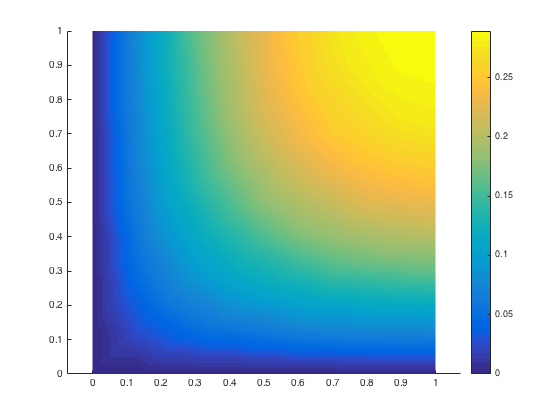
\includegraphics[width=\textwidth]{case1.png}
                \caption{Case 1}
        \end{subfigure}%
        \begin{subfigure}[b]{0.35\textwidth}
                \centering
                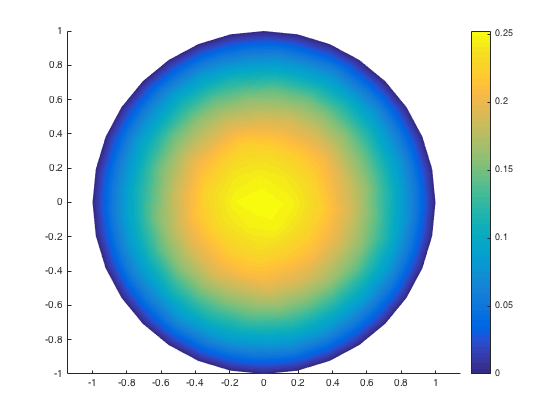
\includegraphics[width=\textwidth]{case2.png}
                \caption{Case 2}
        \end{subfigure}%
        \begin{subfigure}[b]{0.35\textwidth}
                \centering
                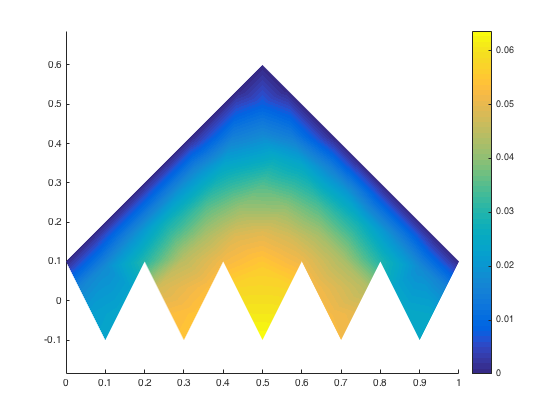
\includegraphics[width=\textwidth]{case3.png}
                \caption{Case 3}
        \end{subfigure}%
        \caption{Finite element solutions \(u_h\) for the three geometries provided in the assignment.}
        \label{fig:5}
\end{figure}

In addition, Fig. \ref{fig:10} shows the solution for a user-defined polygon. 

\begin{figure}[H]
\centering
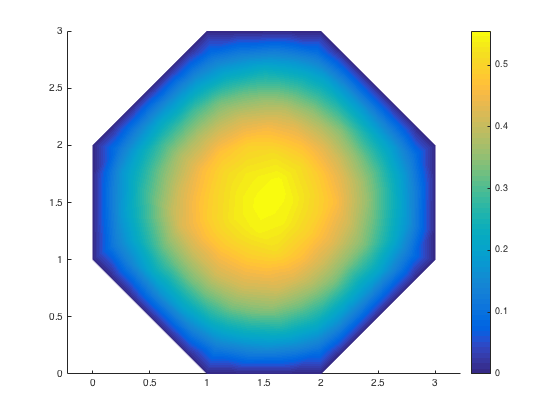
\includegraphics[width=0.5\textwidth]{case4.png}
\caption{Finite element solution \(u_h\) for a fourth geometry.}
\label{fig:10}
\end{figure}

All of the code developed for this section is shown in the Appendix. Not shown are the meshing files developed from the previous homework, since they are largely the same and are still included in the zip file.

\section{}

This problem investigates the convergence properties of the finite element method for linear triangular elements. By solving the same problem with a finer and finer mesh, with the exact solution assumed approximated very well by the finest mesh, the error of each solution with respect to the true solution can be estimated as a function of the mesh refinement. The finer the mesh, the more accurate the solution (as expected due to the higher number of degrees of freedom to capture the behavior), and this investigation will show just how much more accurate the solution is for each successive mesh refinement. This is important knowledge if the tradeoff between more accurate results and longer computation times is a significant factor. 

Fig. \ref{fig:30} and \ref{fig:31} shows the solutions obtained for various levels of refinement for the two problem domains specified. 

\begin{figure}[H]
        \centering
        \begin{subfigure}[b]{0.45\textwidth}
                \centering
                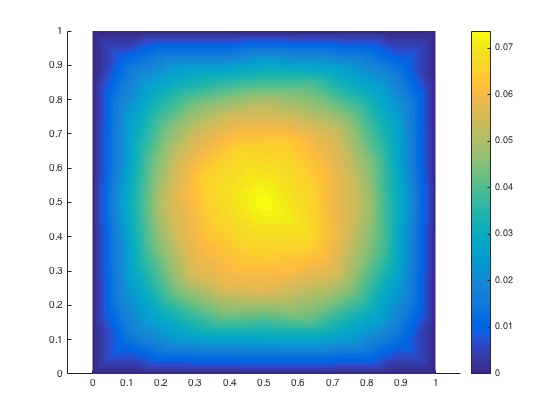
\includegraphics[width=\textwidth]{square0.png}
                \caption{\(n_{ref}=0\)}
        \end{subfigure}%
        \begin{subfigure}[b]{0.45\textwidth}
                \centering
                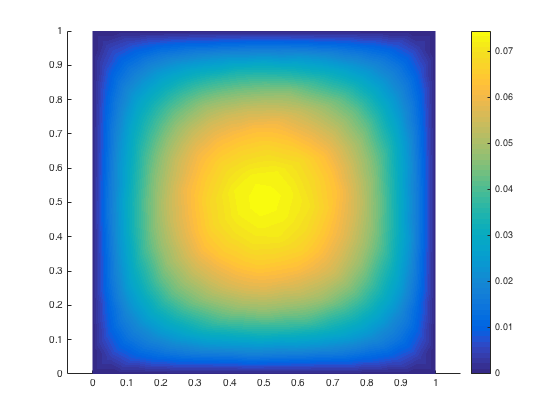
\includegraphics[width=\textwidth]{square1.png}
                \caption{\(n_{ref}=1\)}
        \end{subfigure}\\
        \begin{subfigure}[b]{0.45\textwidth}
                \centering
                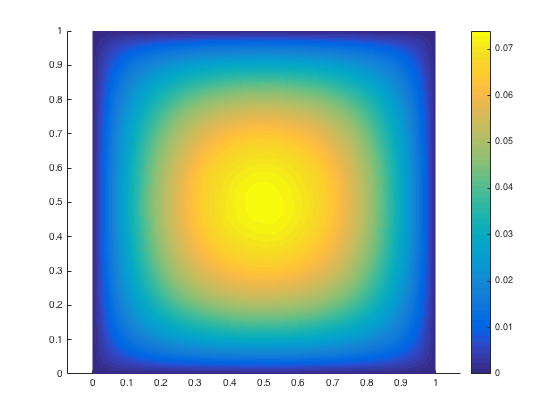
\includegraphics[width=\textwidth]{square2.png}
                \caption{\(n_{ref}=2\)}
        \end{subfigure}%
                \begin{subfigure}[b]{0.45\textwidth}
                \centering
                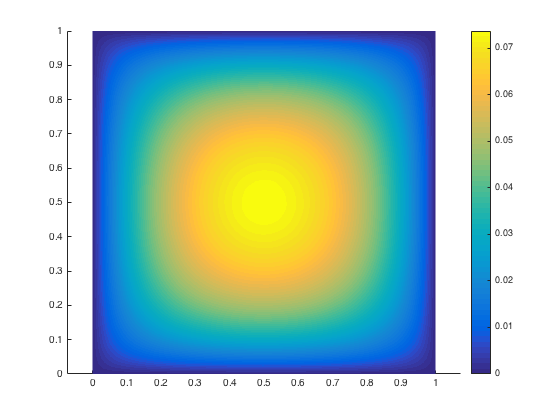
\includegraphics[width=\textwidth]{square3.png}
                \caption{\(n_{ref}=3\)}
        \end{subfigure}%
        \caption{Finite element solutions \(u_h\) for the square geometry provided in the assignment.}
        \label{fig:30}
\end{figure}

\begin{figure}[H]
        \centering
        \begin{subfigure}[b]{0.45\textwidth}
                \centering
                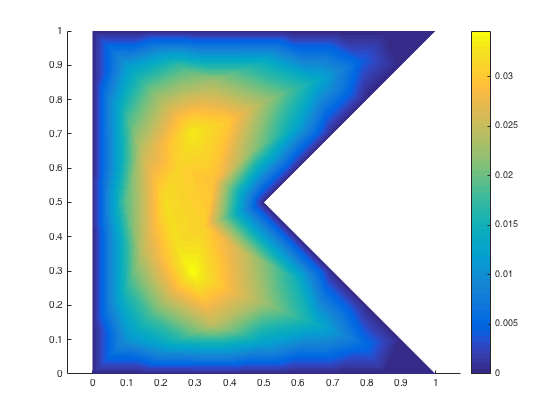
\includegraphics[width=\textwidth]{poly0.png}
                \caption{\(n_{ref}=0\)}
        \end{subfigure}%
        \begin{subfigure}[b]{0.45\textwidth}
                \centering
                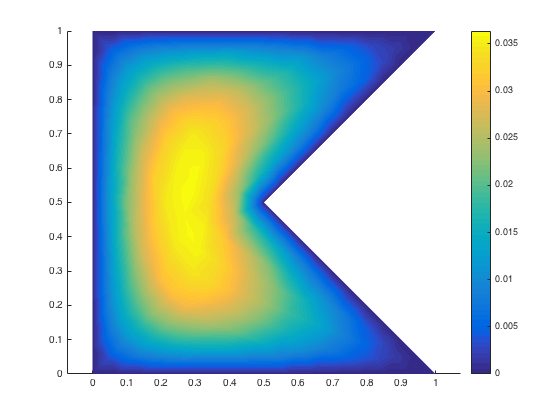
\includegraphics[width=\textwidth]{poly1.png}
                \caption{\(n_{ref}=1\)}
        \end{subfigure}\\
        \begin{subfigure}[b]{0.45\textwidth}
                \centering
                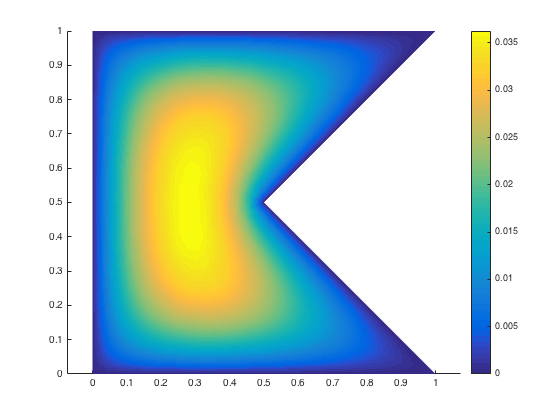
\includegraphics[width=\textwidth]{poly2.png}
                \caption{\(n_{ref}=2\)}
        \end{subfigure}%
                \begin{subfigure}[b]{0.45\textwidth}
                \centering
                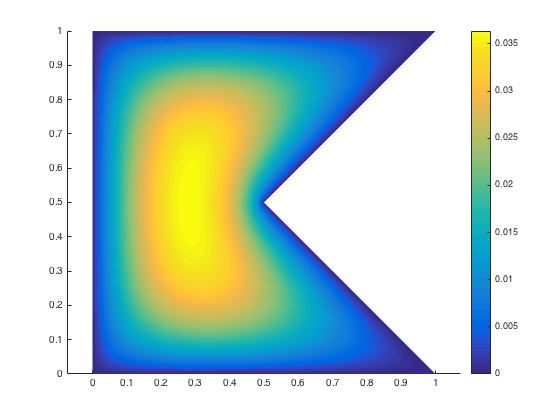
\includegraphics[width=\textwidth]{poly3.png}
                \caption{\(n_{ref}=3\)}
        \end{subfigure}%
        \caption{Finite element solutions \(u_h\) for the polygon geometry provided in the assignment.}
        \label{fig:31}
\end{figure}

The error in each solution is computed as the maximum norm of the errors at the nodes - a loop circulates through all the nodes of the most refined mesh and determines which nodes are shared by the coarser meshes. The maximum norm is defined as the maximum of the absolute difference between the solution values at all the nodes. The slope of these lines on the log-log coordinates is 2.0267 for the square domain and 1.1097 for the polygon domain. This can be interpreted in the following manner - by halving the mesh spacing (as is achieved through a single uniform refinement), the error decreases by a factor of about 2 for the square domain and 1 for the polygonal domain. For linear elements, the finite element method in most situations can be interpreted as being equivalent to a second order finite difference scheme, and so it is to be expected that a convergence rate of 2 be obtained with the square domain. However, some other effect is distorting this convergence rate for the polygonal domain (which we are to talk about soon in lecture, the professor says!).

\section{Appendix}

\subsection{Code, Question 2}

This Python script was used to determine the appropriate Hermite polynomials and the elemental stiffness matrix and elemental load vectors. Because the matrix system reduced to a simple \(2\times 2\) system, the actual solution was performed by hand.

\lstinputlisting[language=Python]{q2.py}

\subsection{Code, Question 3}

Not shown in this document are the meshing files that were submitted with the previous assignment. They are still submitted with this assignment, but there is no reason to include them again.

\subsubsection{\tt fempoi.m}
This function implements the solution of the Poisson equation on an unstructured triangular mesh. 
\lstinputlisting[language=Matlab]{fempoi.m}

\subsubsection{\tt condensation.m}
This function performs static condensation by removing the Dirichlet nodes from the solution so that the correct matrix system can be solved.
\lstinputlisting[language=Matlab]{condensation.m}

\subsubsection{\tt permutation.m}
This function permutes the numbers \(i=1, 2, \cdots, n_{en}\) to be used in filling in the global matrix and vector by the local element matrices and vectors.
\lstinputlisting[language=Matlab]{permutation.m}

\subsection{Code, Question 4}

\subsubsection{\tt poiconv.m}
This function solves a finite element problem for multiple uniform refinement levels and estimates the error as the max-norm of the error at all of the shared nodes between the current refinement level and the maximum refinement level.
\lstinputlisting[language=Matlab]{poiconv.m}

\end{document}
